%----------------------------------------------------------
\def\notedate{2022.12.07}
\def\currentauthor{Василян А.Р. (РК6-73Б)}
%----------------------------------------------------------
\notestatement{rndhpcgui}{Запуск web-приложения на удалённом сервере}

%---------------------------------------------------------

Для запуска на сервере были внесены следующие изменения.

	В файле \textsf{docker-compose.prod} (листинг~\ref{rndhpcgui.2022.12.07.docker-compose.prod}) были изменены порты.

\begin{lstlisting}[frame=single, label={rndhpcgui.2022.12.07.docker-compose.prod}, caption={Содержимое файла \textsf{docker-compose.prod.yml}}, language={docker-compose}] 
	version: '3.8'

	services:
	  web:
		build:
		  context: ./
		  dockerfile: Dockerfile.prod
		command: gunicorn hello_django.wsgi:application --bind 0.0.0.0:8080
		volumes:
		  - static_volume:/home/app/web/staticfiles
		  - media_volume:/home/app/web/mediafiles
		env_file:
		  - ./.env.prod
		depends_on:
		  - db
	  db:
		image: postgres:13.0-alpine
		volumes:
		  - postgres_data:/var/lib/postgresql/data/
		env_file:
		  - ./.env.prod.db
	  nginx:
		build: ./nginx
		volumes:
		  - static_volume:/home/app/web/staticfiles
		  - media_volume:/home/app/web/mediafiles
		ports:
		  - 8084:80
		  - 443:443
		depends_on:
		  - web
	
	volumes:
	  postgres_data:
	  static_volume:
	  media_volume:	
\end{lstlisting}

В файле \textsf{.env.prod}~\ref{rndhpcgui.2022.12.07.env.prod} был изменен хост, на котором будет производиться работа на 195.19.40.68 (localhost сервера, на котором будет запущено приложение).

\begin{lstlisting}[frame=single, label={rndhpcgui.2022.12.07.env.prod}, caption={Содержимое файла \textsf{.env.prod}}, language={aINIExample}] 
	DEBUG=0
	SECRET_KEY=change_me
	DJANGO_ALLOWED_HOSTS=localhost 195.19.40.68 [::1]
	SQL_ENGINE=django.db.backends.postgresql
	SQL_DATABASE=hello_django_prod
	SQL_USER=hello_django
	SQL_PASSWORD=hello_django
	SQL_HOST=db
	SQL_PORT=5432
	DATABASE=postgres
\end{lstlisting}

Больше всего изменений пришлось на файл \textsf{nginx.conf}~\ref{rndhpcgui.2022.12.07.nginx.conf}. 

\begin{lstlisting}[frame=single, label={rndhpcgui.2022.12.07.nginx.conf}, caption={nginx.conf}, language={nginx}] 
	server {
	    listen 80;
	    location /static/ {
	        alias /home/app/web/staticfiles/;
	    }
	    location /media/ {
	        alias /home/app/web/mediafiles/;
	    }
	    location / {
	        proxy_pass http://web:8080;
	        proxy_set_header Host $http_host;
	        proxy_set_header Connection "upgrade";
	        proxy_set_header X-Real-IP $remote_addr;
	        proxy_set_header X-Forwarded-Proto $scheme;
	        proxy_set_header X-Forwarded-For $proxy_add_x_forwarded_for;
	        proxy_set_header Upgrade $http_upgrade;
	        proxy_connect_timeout       600;
	        proxy_send_timeout          600;
	        proxy_read_timeout          600;
	        send_timeout                600;
	    }
	}
\end{lstlisting}

URL-адрес проксируемого сервера устанавливается с proxy_pass директивы proxy_pass и может использовать HTTP или HTTPS качестве протокола, доменного имени или IP-адреса, а также необязательного порта и URI в качестве адреса. Выше в листинге Nginx передает все запросы в '/' прокси-серверу по адресу \url{http://web:8080}.

Чтобы настроить или установить заголовки для прокси-соединений, используется директива proxy_set_header , за которой следует значение заголовка. 
\begin{enumerate}
	\item Connection "upgrade" и Upgrade \$http\_upgrade — эти поля заголовка необходимы, если приложение использует веб-сокеты.
	\item X-Real-IP \$remote_addr — перенаправляет удаленный IP-адрес реального посетителя на прокси-сервер.
	\item X-Forwarded-Proto \$scheme — при использовании внутри блока HTTPS-сервера каждый HTTP-ответ от проксируемого сервера перезаписывается на HTTPS.
	\item X-Forwarded-For \$proxy_add_x_forwarded_for — список, содержащий IP-адреса каждого сервера, через который клиент прошел проксирование.
\end{enumerate}

На рисунке~\ref{rndhpcgui.2022.12.07.picture1} представлен вход на сервер через консоль. 
\begin{figure}[!ht]
  \centering
  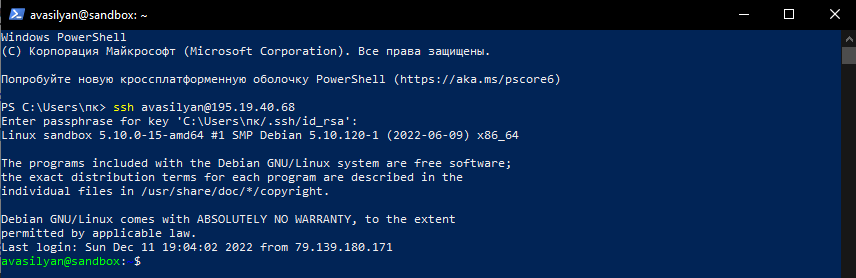
\includegraphics[scale=0.8]{ResearchNotes/rndhpc_dev_gui_2022_12_07/rndhpcgui.2022.12.07.picture1.png}
  \caption{Вход на сервер}\label{rndhpcgui.2022.12.07.picture1}
\end{figure}

Далее в консоли вводятся те же команды для запуска всего приложения, что и ранее. Перейдя по 195.19.40.68:8084, открывается страница, представленная на рисунке~\ref{rndhpcgui.2022.12.07.picture2}, что свидетельствует о корректной работе приложения на удалённом сервере.
\begin{figure}[!ht]
  \centering
  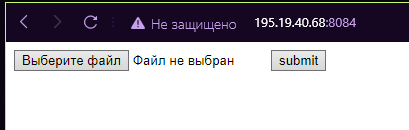
\includegraphics[scale=0.8]{ResearchNotes/rndhpc_dev_gui_2022_12_07/rndhpcgui.2022.12.07.picture2.png}
  \caption{Вход на сервер}
  \label{rndhpcgui.2022.12.07.picture2}
\end{figure}

%----------------------------------------------------------
% Атрибуты задачи
\noteattributes{}
%----------------------------------------------------------
